\documentclass[mathserif,11pt]{beamer}

% Turn off the ugly navigation symbols.
\setbeamertemplate{navigation symbols}{}

% Margins and whatnot.
\setbeamersize{text margin left=1em,text margin right=1em}

% Hoefler Text as the main text font; need to make sure it's happy
% using serif though...
\usepackage{fontspec}
\usefonttheme{serif}
\defaultfontfeatures{Mapping=tex-text} % enable -- / --- / `` / ''
\setmainfont{Hoefler Text}
\setsansfont[BoldFont=Oswald Bold,ItalicFont=Oswald Light]{Oswald}
\newcommand{\amp}{{\fontspec[Alternate=1]{Hoefler Text}\&}}
\newcommand{\QQ}{{\fontspec[Alternate=2]{Hoefler Text}Q}}

\usepackage{tabularx}
\usepackage{array}

\definecolor{verydarkgrey}{HTML}{001112}
\definecolor{fdarkblue}{HTML}{232747}
\definecolor{lightgrey}{HTML}{eeeeee}
\definecolor{grey}{rgb}{0.5, 0.5, 0.5}
\definecolor{darkgreen}{rgb}{0, 0.4, 0} % same as "darkgreen" in R

\setbeamerfont{frametitle}{size=\large}
\setbeamercolor{frametitle}{fg=black}
\setbeamercolor{titleline}{bg=black}
\setbeamercolor{title}{fg=fdarkblue}
\setbeamercolor*{date in head/foot}{fg=verydarkgrey}
\setbeamercolor{item}{fg=fdarkblue}
\setbeamerfont{item}{series=\bfseries}
% Never used, but this is nice.
\setbeamertemplate{itemize subitem}{\normalsize --}

% \useoutertheme{new}

\makeatletter  %Sets category code: http://tex.stackexchange.com/questions/8351/what-do-makeatletter-and-makeatother-do
\usepackage{dashrule}
\defbeamertemplate*{frametitle}{mine}[1][left]
{
  % Increase width of title box
  \@tempdima=\textwidth%
  \advance\@tempdima by\beamer@leftmargin%
  \advance\@tempdima by\beamer@rightmargin%
  %
  \begin{beamercolorbox}[sep=0.3cm,#1,wd=\the\@tempdima]{frametitle}
    \usebeamerfont{frametitle}%
    \vbox{}\vskip-1ex\vspace{.5ex}
    \strut\hspace{1ex}\insertframetitle\strut\par%
    \vskip-1.5ex%
    \hspace{\fill}\hdashrule{\textwidth}{.075ex}{.075ex .2ex}\hspace{\fill}
    \par\nointerlineskip \vspace{\baselineskip}
  \end{beamercolorbox}%
  \nointerlineskip%
  \vspace{-1ex}
}

\setbeamercolor*{date in head/foot}{bg=black,fg=white}







\usepackage{tikz}
\usetikzlibrary{positioning}
\usetikzlibrary{calc}
\usetikzlibrary{arrows,positioning, decorations, decorations.text}

% Define new environment for overlaying transparent text box, eg.g. for title
\usepackage[framemethod=tikz]{mdframed}
\newmdenv[tikzsetting={draw=black,fill=white,fill opacity=0.7, line width=4pt, rounded corners, inner sep=10pt, inner ysep=10pt},backgroundcolor=none,leftmargin=0,rightmargin=0,innertopmargin=4pt,skipbelow=\baselineskip,%
skipabove=\baselineskip]{TitleBox}

% macro for small text at lower right of screen, e.g. links
\usepackage[overlay,absolute]{textpos}
\newcommand\FrameText[1]{
  \begin{textblock*}{\paperwidth}(0pt,.98\textheight)
    \raggedleft \small  #1\hspace{.5em}
  \end{textblock*}}

% some formatting options for green blue slide
\tikzstyle{greenblue_bodytext} = [text width=.45\paperwidth,text badly ragged,  rounded corners, inner sep=10pt, inner ysep=10pt, fill=white, line width=2pt]

% Defines a command to make two new slides with different backgorunds,
% place two text boxes on page n top left and bottom right,

\newcommand{\greenblueslide}[6]{%
\begin{frame}[empty]
   \begin{tikzpicture}[remember picture,overlay]
     \node at (current page.center) {
       \includegraphics<1>[width=\paperwidth]{#1}
       \includegraphics<2>[width=\paperwidth]{#4}
     };
     \node[draw,anchor=north west, greenblue_bodytext, draw= green] at
       ($(current page.north west) + (.05\paperwidth, -.1\paperheight)$)
       {{\bf Plants: }\\ {\small #2}};

     \only<2>{
     \node[draw,anchor=south east, greenblue_bodytext, draw=blue] at
       ($(current page.south east) - (.05\paperwidth, -.1\paperheight)$)
       {{\bf Marine: }\\ {\small #5}};
       }
   \end{tikzpicture}
   \only<1>{ \FrameText{ {\color{grey} #3}}}
   \only<2>{ \FrameText{ {\color{grey} #6}}}
\end{frame}
}

\newcommand{\traitsummary}[9]{

\tikzstyle{boxStyle1}=[anchor = center, rectangle, rounded corners, thick, inner sep=4pt, inner ysep=4pt, align = center, fill =white, text width = 3cm]
\tikzstyle{boxStyle2}=[boxStyle1, text width = 8cm]

% define styles - lines
\tikzstyle{lineStyle1}=[shorten <=2pt, shorten >=2pt]

  % anchor
  \node[] at ($(current page.center) + (0, 3cm)$) (middle){};
  % top row
   \node[boxStyle1, left = 3cm of middle.center, text = darkgreen] (low) { #1  };
   \node[boxStyle1, right = 3cm of middle.center, text = darkgreen] (high) { #3 }
      edge [<->, line width = 5pt, lineStyle1, draw=darkgreen!50]                  (low);
  \node[boxStyle1 , draw = black, text width = 3cm] at (middle) {\large #2};
  % second row
  \node[boxStyle2, below = 0.8cm of middle.center, text = black!50] (middle2) {\small (direct physiological trade-off)};
   \node[boxStyle1, left = 3cm of middle2.center] (low2) {\small #4};
   \node[boxStyle1, right = 3cm of middle2.center] (high2) {\small #5};
  % 3rd row
  \node[boxStyle2, below =0.8cm of middle2.center, text = black!50] (middle3) {\small (functional outcome)};
   \node[boxStyle1, left = 3cm of middle3.center, text = black] (low3) {\small #6};
   \node[boxStyle1, right = 3cm of middle3.center, text = black] (high3) {\small #7};
 % 4th row
  \node[boxStyle2, below =0.8cm of middle3.center, text = black!50] (middle4) {\small (demographic outcome)};
   \node[boxStyle1, left = 3cm of middle4.center, text = black] (low4) {\small #8};
   \node[boxStyle1, right = 3cm of middle4.center, text = black] (high4) {\small #9};

}


% From Rich - macro for???
\makeatother   % Sets category code: http://tex.stackexchange.com/questions/8351/what-do-makeatletter-and-makeatother-do
\usepackage{relsize}
\newenvironment{tframe}{
  \begin{frame}[plain]
    \begin{tikzpicture}[remember picture,overlay]
      \node[at=(current page.center)] {
        \includegraphics[width=\paperwidth]{pics/purple-gradient-background}
      };
    \end{tikzpicture}
    \color{white}
    \sf\relsize{3}}
    {\end{frame}}



\usepackage{fontspec}
\usepackage{slides/modules/tex/fontawesome} % nice glyphs
\usepackage{tikz}

\definecolor{macouleur1}{HTML}{E41A1C}
\definecolor{macouleur2}{HTML}{377EB8}
\definecolor{macouleur3}{HTML}{4DAF4A}
\definecolor{macouleur4}{HTML}{984EA3}
\definecolor{macouleur5}{HTML}{FF7F00}
%% \setbeamerfont{frametitle}{size=\Large}

\title{How shifts in traits composition along climatic gradients emerge
  from the interplay of climate stress and competition? A theoretical
  model analysis in forests.}
\author{Georges Kunstler (Irstea) \\ Daniel Falster (Macquarie University) \\ Rich Fitzjohn (Macquarie University)}
\date{{SFecologie, 25-27/10/2016, Marseille}}
\institute[\href{mailto: georges.kunstler@irstea.fr}{ { \FA \faEnvelope} georges.kunstler@irstea.fr}]{}

%----------------------------------------------------------------------------------------
\begin{document}
%----------------------------------------------------------------------------------------

{
 \begin{frame}[plain]
  % \vspace*{1em}
  \begin{TitleBox}
  {\LARGE \inserttitle} \vskip2pt
  {\footnotesize \insertdate}
 \end{TitleBox}
 \begin{TitleBox}[rightmargin=40, tikzsetting={draw=black,fill=white,fill opacity=0.7, line width=2pt}]
  \insertauthor \\
  {\footnotesize \insertshortinstitute
  }
 \end{TitleBox}
\begin{tikzpicture}[remember picture, overlay]
   \node[anchor = center] at ($(current page.center) + (2.5cm, -1.6cm)$) (image) {
    
\includegraphics[width=0.15\paperwidth]{slides/image/IRSTEA_LOGO_cmjn_200px.jpg}};
  \end{tikzpicture}

 \end{frame}
}

%% %-----------------------------------


\section{intro}

%-----------------------------------

\begin{frame}\frametitle{\textbf{Interplay between abiotic constrains
      and competition}}
\begin{tikzpicture}[remember picture, overlay]
  \node[anchor = west, align = center, text width=13cm] at ($(current page.west) + (-0.5cm, 0.5cm)$) {
      \begin{itemize} \itemsep 6pt \parskip0pt
         \item[]\textbf{Plant species composition shift along
             abiotic gradients and species ranges:}
        \begin{itemize} \itemsep 6pt \parskip0pt
           \item[]<2->\textbf{$\Rightarrow$ species physiological
             tolerance to climate stresses}
           \item[]<3->\textbf{{\color{red}$\Rightarrow$ but also biotic interactions (such as competition)}}
           \item[]<4->\textbf{{\color{red} Two visions of the role of competition}}
        \end{itemize}
      \end{itemize}
     };
   \end{tikzpicture}
\end{frame}


% %-------------

\begin{frame}\frametitle{\textbf{Classical view: Fundamental niche differentiation}}
 \begin{tikzpicture}[remember picture, overlay]
   \node[anchor = center] at ($(current page.center) + (1.5cm, -0.5cm)$) (image) {
    \includegraphics[width=0.65\paperwidth]<1->{figures/resLV_0a.pdf}
};
 \node[anchor = west, align = center, text width=4.5cm] at ($(current
  page.west) + (-0.7cm, 1.5cm)$) {
        \begin{itemize} \itemsep 6pt \parskip0pt
           \item[]<2-> {\color{red} $\Rightarrow$ \textbf{Dominant in
                 the litterature}}
        \end{itemize}
};
 \end{tikzpicture}
\end{frame}


\begin{frame}\frametitle{\textbf{Alternative view: Shifting
      competitive hierarchy}}
 \begin{tikzpicture}[remember picture, overlay]
   \node[anchor = center] at ($(current page.center) + (1.5cm, -0.5cm)$) (image) {
    \includegraphics[width=0.65\paperwidth]<1->{figures/resLV_0b.pdf}
     };
 \node[anchor = west, align = center, text width=4.5cm] at ($(current
  page.west) + (-0.7cm, 1.5cm)$) {
        \begin{itemize} \itemsep 6pt \parskip0pt
           \item[]<2->\textbf{Tradeoff between competitive ability
                    \textit{vs.} stress tolerance}
           \item[]<3-> {\color{red} $\Rightarrow$ \textbf{Few studies in the litterature}}
        \end{itemize}

};
 \end{tikzpicture}
\end{frame}


%-----------------------------------

\begin{frame}\frametitle{\textbf{Studies testing a tradeoff between competitive ability
                    \textit{vs.} climate stress tolerance in trees?}}
\begin{tikzpicture}[remember picture, overlay]
  \node[anchor = west, align = center, text width=13cm] at ($(current page.west) + (-0.5cm, 2.5cm)$) {
      \begin{itemize} \itemsep 6pt \parskip0pt
         \item[]<2->\textbf{Trade-off between maximum height growth and
             frost tolerance (Hoehler \textit{et al.} 2012 based on the seminal idea of Loehle 1998)}
      \end{itemize}
    };
   \node[anchor = center] at ($(current page.center) + (0cm, -1.2cm)$) (image) {
    \includegraphics[width=0.7\paperwidth]<2->{slides/image/tradefrost.png}
     };
   \end{tikzpicture}
\end{frame}

%-----------------------------------

\begin{frame}\frametitle{\textbf{Studies testing a tradeoff between competitive ability
                    \textit{vs.} climate stress tolerance in trees?}}
\begin{tikzpicture}[remember picture, overlay]
  \node[anchor = west, align = center, text width=13cm] at ($(current page.west) + (-0.5cm, 2.5cm)$) {
      \begin{itemize} \itemsep 6pt \parskip0pt
         \item[]\textbf{Trade-off between shade tolerance and
             frost tolerance (Lusk et al. 2013) }
      \end{itemize}
     };
   \node[anchor = center] at ($(current page.center) + (0cm, -1.1cm)$) (image) {
    \includegraphics[width=0.6\paperwidth]<1>{slides/image/tradeshade.png}
    };
   \end{tikzpicture}
\end{frame}


%-----------------------------------

\begin{frame}\frametitle{\textbf{Competitive ability vs. climate
      tolerance tradeoff consequences in forests}}
\begin{tikzpicture}[remember picture, overlay]
  \node[anchor = west, align = center, text width=13cm] at ($(current page.west) + (-0.5cm, 0cm)$) {
      \begin{itemize} \itemsep 6pt \parskip0pt
         \item[] <1-> Competitive ability in both \large{\textbf{early
               successional} and \textbf{late successional} stages} can tradeoff against climate stress tolerance
         \item[]<2-> Objectives of this talk
         \item[]<3-> 1. Consequence of such
           tradeoff on community structure in a theoretical model
         \item[]<4-> 2. Explore one trait-based physiological
           mecanisms that can lead to such tradeoff and its
           evolutionary consequences on community assembly
      \end{itemize}
     };
\end{tikzpicture}
\end{frame}

%----------------------------------
\begin{frame}\frametitle{\textbf{Theoretical model:
      successional niche}}
\begin{tikzpicture}[remember picture, overlay]
   \node[anchor = center] at ($(current page.center) + (0cm, -0.3cm)$) (image) {
    \includegraphics[width=1\paperwidth]<2>{slides/image/Pacala.png}
    };
   \end{tikzpicture}
\end{frame}

%----------------------------------

\begin{frame}\frametitle{\textbf{Successional niche: 2 theoretical traits}}
\begin{tikzpicture}[remember picture, overlay]
  \node[anchor = center] at ($(current page.center) + (0cm, 0cm)$) (image) {
    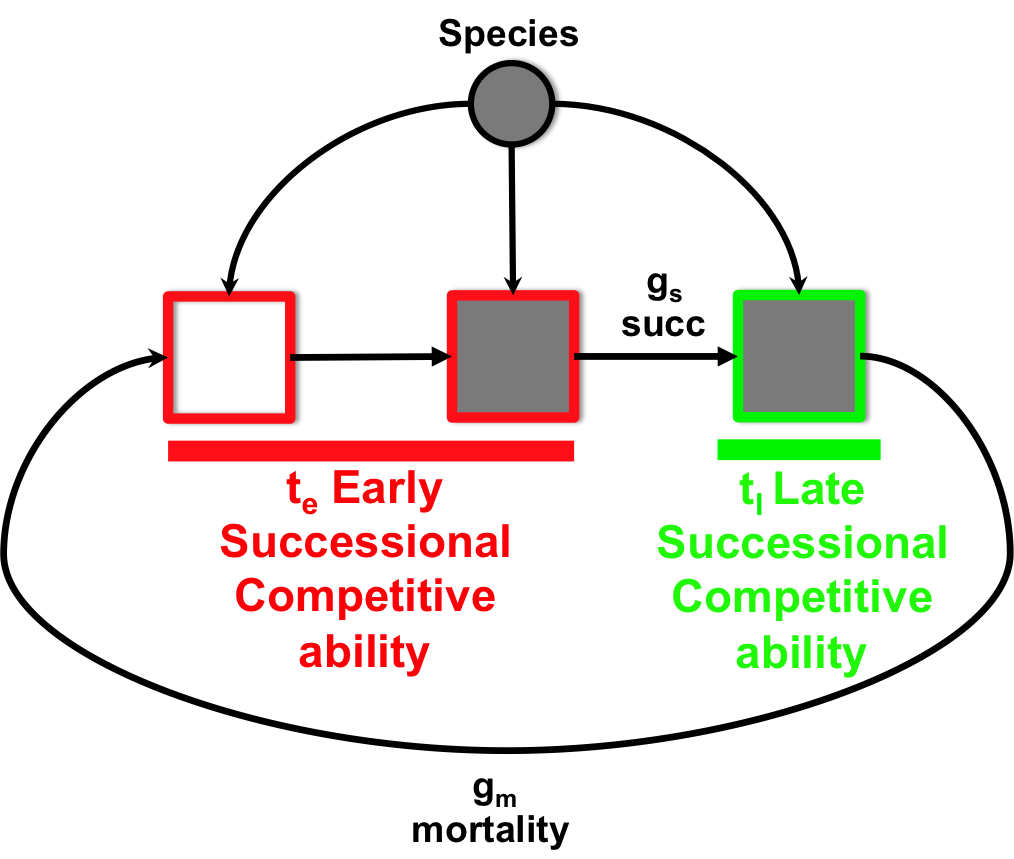
\includegraphics[width=0.62\paperwidth]{slides/image/succ.png}
    };
\end{tikzpicture}
\end{frame}


\begin{frame}\frametitle{\textbf{Cellular automaton (gradient of
      stress and local dispersal)}}
\begin{tikzpicture}[remember picture, overlay]
  \node[anchor = center] at ($(current page.center) + (0cm, 0cm)$) (image) {
    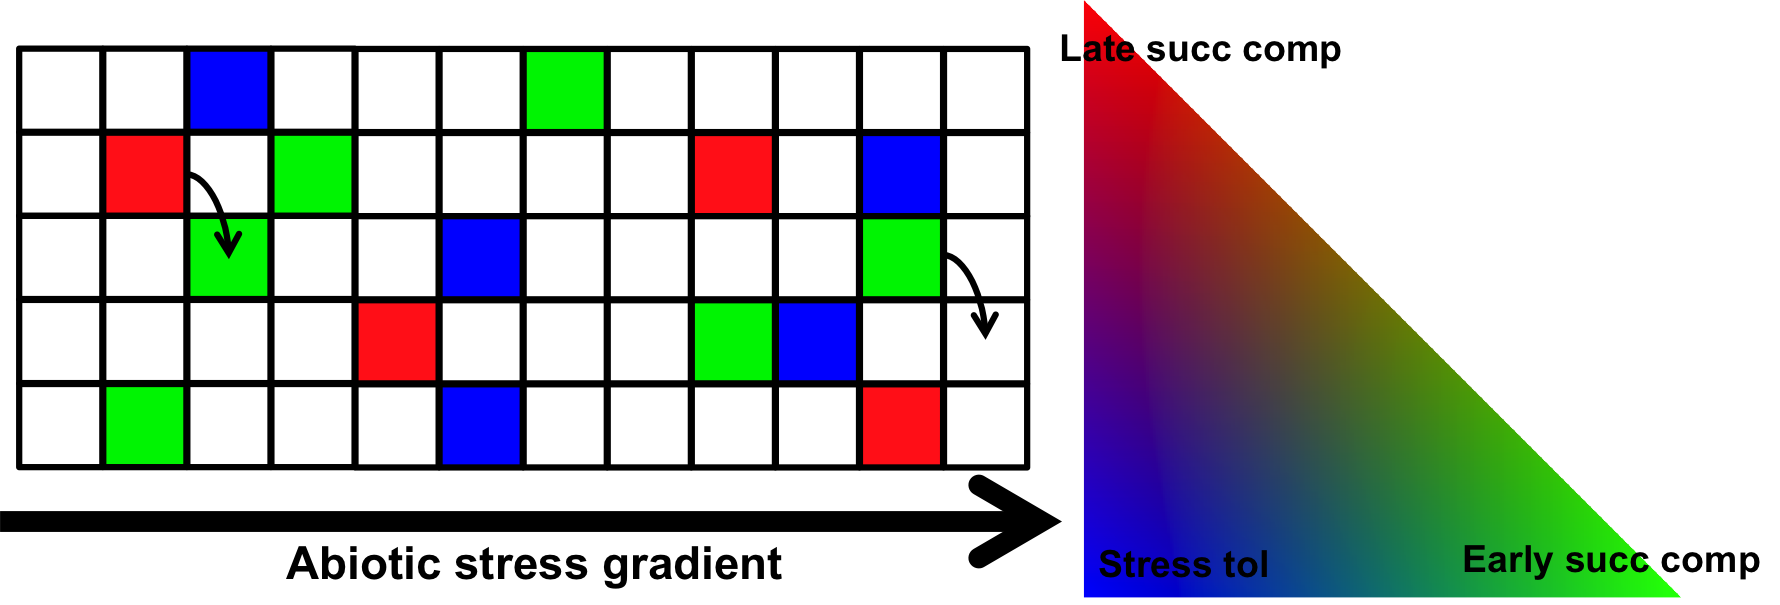
\includegraphics[width=1\paperwidth]{slides/image/auto.png}
    };
\end{tikzpicture}
\end{frame}


%----------------------------------
\begin{frame}\frametitle{\textbf{Pattern along abiotic stress gradient}}
\begin{tikzpicture}[remember picture, overlay]
   \node[anchor = center] at ($(current page.center) + (0cm, 2cm)$) (image) {
    \includegraphics[width=1\paperwidth]<1>{slides/image/maps_gradients100.pdf}
    };
   \node[anchor = center] at ($(current page.center) + (0cm, -1.5cm)$) (image) {
    \includegraphics[width=0.3\paperwidth]{slides/image/3dtrade_offRGB.pdf}
    };

   \end{tikzpicture}
\end{frame}


%-----------------------------------

\begin{frame}\frametitle{\textbf{Match a key pattern observed in
      tree communities}}
\begin{tikzpicture}[remember picture, overlay]
  \node[anchor = west, align = center, text width=11cm] at ($(current page.west) + (0.5cm, 3.2cm)$) {
      \begin{itemize} \itemsep 6pt \parskip0pt
         \item<1->\textbf{Increasing abundance of early-successional species
           with latitude (Morin \& Chuine 2006)}
      \end{itemize}
     };
   \node[anchor = center] at ($(current page.center) + (-0.5cm, -0.7cm)$) (image) {
    \includegraphics<3>[width=0.6\paperwidth]{slides/image/early_gradients100.pdf}
    \includegraphics<2>[width=0.6\paperwidth]{slides/image/morin.png}
    };
   \end{tikzpicture}
\end{frame}


% \begin{frame}\frametitle{\textbf{Match several patterns observed in
%       tree communities}}
% \begin{tikzpicture}[remember picture, overlay]
%   \node[anchor = west, align = center, text width=11cm] at ($(current page.west) + (0.5cm, 3.2cm)$) {
%       \begin{itemize} \itemsep 6pt \parskip0pt
%          \item<1->\textbf{Rapoport’s rule: species in low stress areas
%              have smaller ranges}
%       \end{itemize}
%      };
%    \node[anchor = center] at ($(current page.center) + (-0.5cm, -0.7cm)$) (image) {
%     \includegraphics<2>[width=0.5\paperwidth]{slides/image/morin2.png}
%     \includegraphics<3>[width=0.6\paperwidth]{slides/image/range_gradients100.pdf}
%     };
%    \end{tikzpicture}
% \end{frame}

%-----------------------------------

\begin{frame}\frametitle{\textbf{Theoretical model not connected with real traits}}
\end{frame}


%----------------------------------
\begin{frame}\frametitle{\textbf{Plant: a trait based physiological
      model of metacommunities. Falster \textit{et al.} (2016) MEE}}
\end{frame}

% \begin{frame}{Individual-based model $\rightarrow$ rules about plant function}
%   \begin{center}
%    \includegraphics<1>[height=.8\textheight]{slides/image/plantmodel-7}
%   \end{center}
%  \FrameText{ \color{red}slide D. Falster}
% \end{frame}

\begin{frame}{\textbf{Plant: Size-structured physiological demographic model}}
\begin{tikzpicture}[remember picture, overlay]
   \node[anchor = center] at ($(current page.center) + (0cm,0cm)$) (image) {
   \includegraphics<1>[height=.8\textheight]{slides/image/blackbox.pdf}
    };
   \end{tikzpicture}
 \FrameText{ \color{red}slide D. Falster}
\end{frame}

% NOTES:
\begin{frame}{\textbf{Plant: Size structured metacommunity}}
\begin{tikzpicture}[remember picture, overlay]
   \node[anchor = center] at ($(current page.center) + (0cm, 0cm)$) (image) {
   \includegraphics<1>[height=.8\textheight]{slides/image/patch-4}
    };
   \end{tikzpicture}
 \FrameText{ \color{red}slide D. Falster}
\end{frame}


%-----------------------------------

\begin{frame}\frametitle{\textbf{Plant: Leaf Mass per Area (LMA) a key traits
      for successional niches (Falster et al. (2015) BioRxiv)}}
\begin{tikzpicture}[remember picture, overlay]
  \node[anchor = west, align = center, text width=11cm] at ($(current page.west) + (0cm, 2.1cm)$) {
      \begin{itemize} \itemsep 6pt \parskip0pt
         \item<2->  LMA $\rightarrow$ shade-tolerance
           \textit{vs.} high light tradeoff
         \item<3->  Evolutionary stable strategies ESS of LMA $\rightarrow$
           coexistence through successional niche
      \end{itemize}
     };
   \node[anchor = center] at ($(current page.center) + (0cm, 0cm)$) (image) {
    \includegraphics[width=0.8\paperwidth]<1>{slides/image/LMA.png}
    };
   \node[anchor = center] at ($(current page.center) + (0cm, -0.8cm)$) (image) {
    \includegraphics[width=0.65\paperwidth]<2>{figures/tradeoff_shade_light.pdf}
    };
   \node[anchor = center] at ($(current page.center) + (0cm, -1.7cm)$) (image) {
    \includegraphics[width=0.6\paperwidth]<3>{slides/image/fitness_lma.png}
    };
   \end{tikzpicture}
\end{frame}


% %-----------------------------------

% \begin{frame}\frametitle{\textbf{Predictons along a gradient of stress
%     (Amax)}}
% \begin{tikzpicture}[remember picture, overlay]
%    \node[anchor = center] at ($(current page.center) + (0cm, 0cm)$) (image) {
%    \includegraphics<2>[height=1\textheight]{figures/gradient_lma_multi.pdf}
%     };
%    \end{tikzpicture}
%  \FrameText{ \color{red}see Falster et al. (2015) BioRxiv}
% \end{frame}

%-----------------------------------

\begin{frame}\frametitle{\textbf{Traits related to stress tolerance?}}
\end{frame}



%----------------------------------
\begin{frame}\frametitle{\textbf{Leaf N to compensate low water availability}}
\begin{tikzpicture}[remember picture, overlay]
  \node[anchor = center, align = center, text width=11cm] at ($(current page.center) + (0cm, 2.3cm)$) {
      \begin{itemize} \itemsep 6pt \parskip0pt
         \item[]<2-> $\rightarrow$  clear pattern of increase of Leaf
           N with aridity (Reich \& Oleksyn 2004)
         \item[]<3-> $\rightarrow$  Leaf level model proposed by Wright et al. (2003)
      \end{itemize}
     };
   \node[anchor = center] at ($(current page.center) + (0cm, -1.6cm)$) (image) {
    \includegraphics[width=0.95\paperwidth]<3>{slides/image/Wright.png}
      };
   \end{tikzpicture}
\end{frame}

%-----------------------------------

\begin{frame}\frametitle{\textbf{Implementation of Leaf N in `Plant` photosynthesis}}
\begin{tikzpicture}[remember picture, overlay]
   \node[anchor = center] at ($(current page.center) + (2.2cm, 0cm)$) (image) {
   \includegraphics<2->[height=1\textheight]{figures/WaterS_LeafN_contour.pdf}
    };
 \node[anchor = west, align = center, text width=4.5cm] at ($(current
  page.west) + (-.5cm, 2cm)$) {
        \begin{itemize} \itemsep 6pt \parskip0pt
           \item<3-> {\textbf{Leaf N compensate
            ardity}}
           \item<4-> {\textbf{but respiration cost}}
        \end{itemize}
};

   % \node[anchor = center] at ($(current page.center) + (0cm, 0cm)$) (image) {
   % \includegraphics<3>[height=1\textheight]{figures/WaterS_LeafN.pdf}
   %  };
   \end{tikzpicture}
\end{frame}

%-----------------------------------

%-----------------------------------

\begin{frame}\frametitle{\textbf{ESS of LMA and Narea along a gradient of water stress}}
% \begin{tikzpicture}[remember picture, overlay]
%    \node[anchor = center] at ($(current page.center) + (-0.5cm, -0.5cm)$) (image) {
%    \includegraphics<1>[height=0.9\textheight]{figures/gradient_narea_lma_multi_narea_lma2.pdf}
%     };
%    \end{tikzpicture}
\begin{tikzpicture}[remember picture, overlay]
   \node[anchor = center] at ($(current page.center) + (0cm, 0cm)$) (image) {
   \includegraphics<2>[height=1\textheight]{figures/gradient_narea_lma_multi_narea_lma.pdf}
    };
   \end{tikzpicture}
\end{frame}


\begin{frame}\frametitle{\textbf{Pattern along gradient of water
      stress in `Plant`}}
\begin{tikzpicture}[remember picture, overlay]
  \node[anchor = center, align = center, text width=11cm] at ($(current page.center) + (0cm, 0cm)$) {
      \begin{itemize} \itemsep 6pt \parskip0pt
         \item<1-> \textbf{Low Narea only at low water stress levels}
         \item<1-> Low Narea with high LMA => shade-tolerant species
         \item<2-> \textbf{But high Narea at both low and high water stress levels}
         \item<2-> No clear tradeoff with hight-light height growth
           (early successional)
      \end{itemize}
     };
   \end{tikzpicture}
\end{frame}

%----------------------------------
\begin{frame}\frametitle{\textbf{Discussion}}
\begin{tikzpicture}[remember picture, overlay]
  \node[anchor = center, align = center, text width=11cm] at ($(current page.center) + (0cm, 0cm)$) {
      \begin{itemize} \itemsep 6pt \parskip0pt
         \item<1-> \textbf{Tradeoffs between competitive ability and
             climate stress tolerance connected to important
             biogeographic patterns}
         \item<2-> Traits $\rightarrow$ tradeoff between climate stress
           tolerance and both early- and late-
           successional competitive abilities?
         \item<3-> Other traits
      \begin{itemize} \itemsep 6pt \parskip0pt
         \item<3-> Vessel size and frost tolerance
         \item<3-> P50 and drought tolerance
      \end{itemize}
         \item<4-> Need more test of such tradeoff with field data
      \end{itemize}
     };
   \end{tikzpicture}
\end{frame}

%----------------------------------
\begin{frame}\frametitle{\textbf{Thanks to ....}}
\begin{tikzpicture}[remember picture, overlay]
  \node[anchor = center, align = center, text width=11cm] at ($(current page.center) + (0cm, 2.5cm)$) {
      \begin{itemize} \itemsep 6pt \parskip0pt
         \item<1-> \textbf{my co-authors D. Falster and
             R. FitzJohn}
         \item<1-> \textbf{and also to M. Westoby (Macquarie
             University) for discussion on this topic}
      \end{itemize}
     };
   \node[anchor = center] at ($(current page.center) + (-2.3cm, 0cm)$) (image) {
   \includegraphics[height=0.3\textheight]<1->{slides/image/daniel.png}
    };
   \node[anchor = center] at ($(current page.center) + (2.3cm, 0cm)$) (image) {
   \includegraphics[height=0.3\textheight]<1->{slides/image/rich.png}
    };
   \node[anchor = center] at ($(current page.center) + (0cm, -3cm)$) (image) {
   \includegraphics[height=0.3\textheight]<1->{slides/image/mark.png}
    };
   \end{tikzpicture}
\end{frame}

\end{document}
